\subsubsection{Dynamics in scene}
In the current experimental SPC setup the exposure time is between 10 to 50 seconds which increases the chance of dynamics in the scene. Dynamics in the scene will reduce the reconstruction performance because the signal is assumed to be constant. By simulating dynamics in a controlled environment the measured signal characteristics for different cases can be identified. Dynamics in the scene can roughly be roughly divided into two separate categories, luminance change and movement. In this section global luminance change and two kinds of motion be simulated. The goal is to interpret how the signal change and if it can be suppressed for better reconstruction.\\[0.1in]




In the first scenario a object is placed in an image but for each measurement the location of the object will be moved in a bounded area of the image. This model represents a scene where the background is static but a person is standing in the same area but moves around.



\begin{figure}[H]
    \centering
\begin{minipage}[t]{0.53\textwidth}
    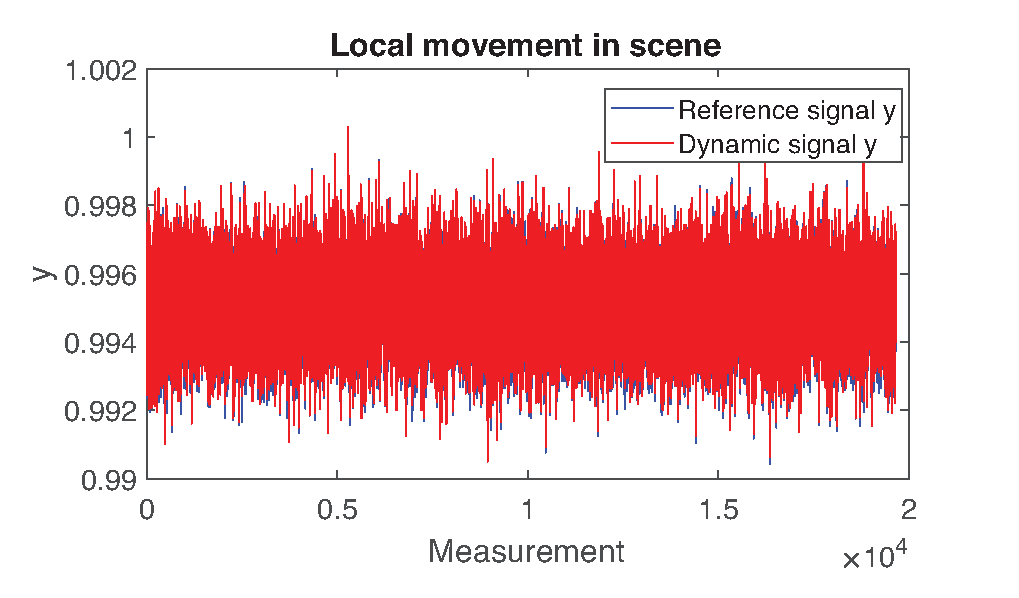
\includegraphics[width=1\textwidth]{result/dynamic/local/local_whole_time1.eps}
    \subcaption{}
    \label{fig:local_sig_1}
\end{minipage}
\begin{minipage}[t]{0.46\textwidth}
    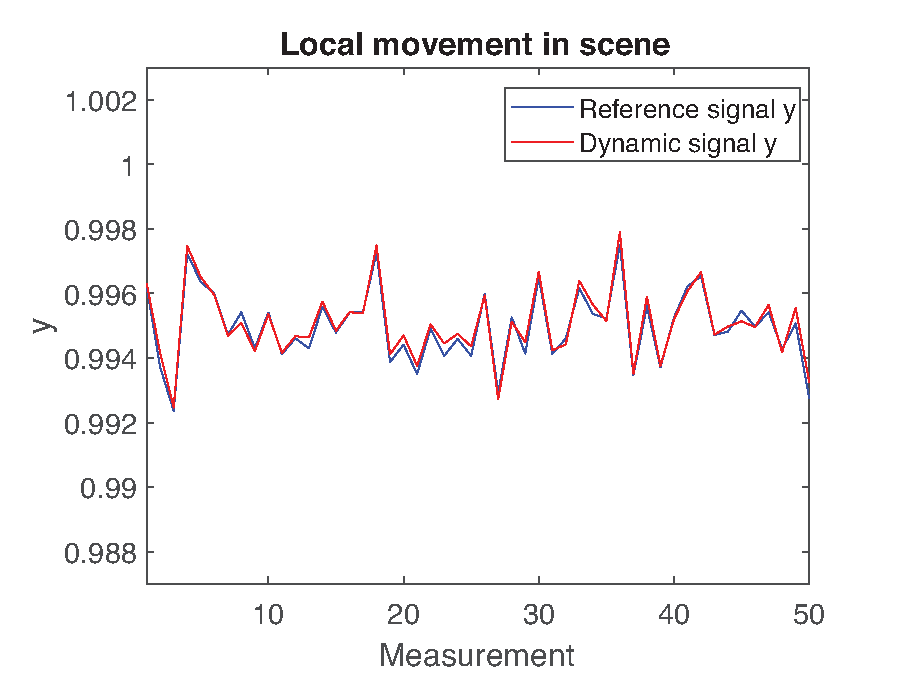
\includegraphics[width = \textwidth]{result/dynamic/local/local_whole_time_win1.eps}
    \subcaption{}
    \label{fig:local_sig_2}
\end{minipage}
    \caption{(a) Pertubated signal from local movement on top of reference signal. (b) Zoomed in view of some samples from figure (a).}
    \label{fig:local_sig}
\end{figure}

As seen in figure~\ref{fig:local_sig_1} there is no obvious difference between the non perturbed reference signal and the distorted signal. In figure~\ref{fig:local_sig_2} where some of the samples is displayed no large difference can be seen either. It can be interpreted as added noise to the signal and it is barely detectable even if the signal is known.\\[0.1in]

The reconstructed images from the reference signal and the perturbed signal is displayed in figure~\ref{fig:local_2} and \ref{fig:local_3} respectively. The difference between the reconstructed images is visible to the naked eye, not only does the object moving around get blurry and noisy but the whole image globally.


\begin{figure}[H]
    \centering
\begin{minipage}[t]{0.32\textwidth}
    
\includegraphics[width=1\textwidth]{result/dynamic/local/local_whole_time_org.png}
    \subcaption{}
    \label{fig:local_1}
\end{minipage}
\begin{minipage}[t]{0.32\textwidth}
    
\includegraphics[width = \textwidth]{result/dynamic/local/local_whole_time_ref.png}
    \subcaption{}
    \label{fig:local_2}
\end{minipage}
\begin{minipage}[t]{0.32\textwidth}
    
\includegraphics[width = \textwidth]{result/dynamic/local/local_whole_time_res_psnr_29_snr_25_sssim_91.png}
    \subcaption{}
    \label{fig:local_3}
\end{minipage}
    \caption{The results of local movement on a reconstructed image, sub sampled at 30\%. (a) Original reference image. (b) Reference image reconstructed from the original image without movement. (c) Reconstructed image from a scene with local movement.}
    \label{fig:local_dyn}
\end{figure}

In table~\ref{tab:local_dyn} the results from calculating PSNR and SSIM between the reconstructed images is presented. It can be observed that the image has been effected to some degree by the movement.

\begin{table}[H]
    \centering
  \begin{tabular}{ | l | l |}
    \hline
    Peak SNR  & SSIM \\ \hline
    29  & 91 \\ 
    \hline
  \end{tabular}
      \caption{Effects comparing non perturbed reconstructed image against reconstructed image with local movement}
    \label{tab:local_dyn}
\end{table}


The conclusion of this test implies that local movement in a scene will cause noise in the image globally and especially locally where the movement occurred. It also implies that local movement is very hard to detect in the signal even if a reference signal is available.\\[0.1in] 



%%%%%%%%%% Second scenario %%%%%%%%%%%%%%%%

The second scenario is an object passing through, moves out or moves to an other place in the scene far from the original place. The problem is modeled with a static background then as the simulated measurement is acquired the object will cross the scene, like a car, human or animal might do when using the SPC. The object will cross the scene in 1000 measurements of approximately 19000 which corresponds to approximately $0.7$ seconds when sampling measurements with the SPC in its current setup.\\[0.1in]



\begin{figure}[H]
    \centering
\begin{minipage}[t]{0.53\textwidth}
    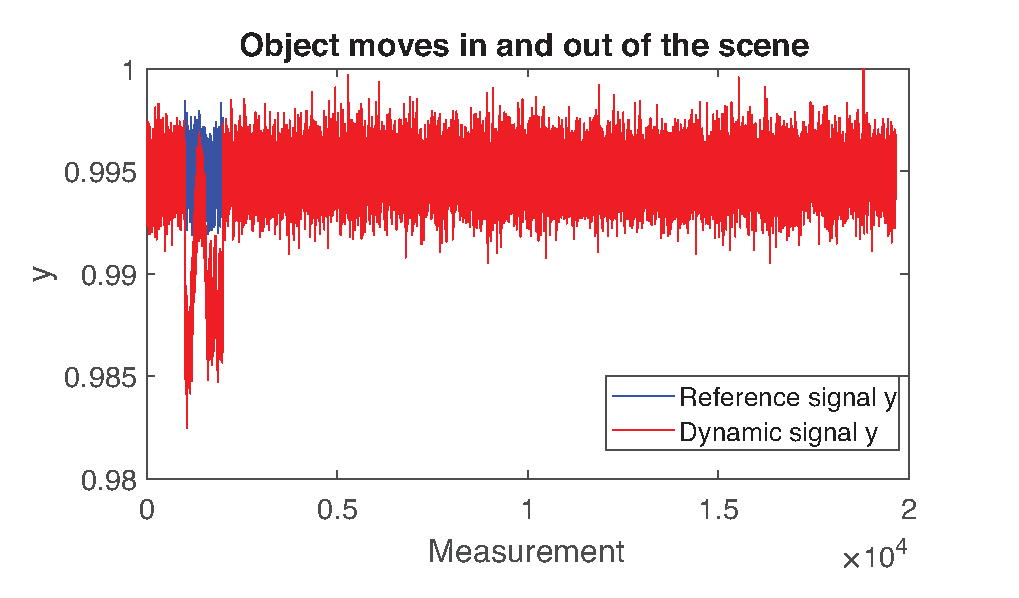
\includegraphics[width=1\textwidth]{result/dynamic/fly/flyby_sig1.eps}
    \subcaption{}
    \label{fig:fly_sig_1}
\end{minipage}
\begin{minipage}[t]{0.46\textwidth}
    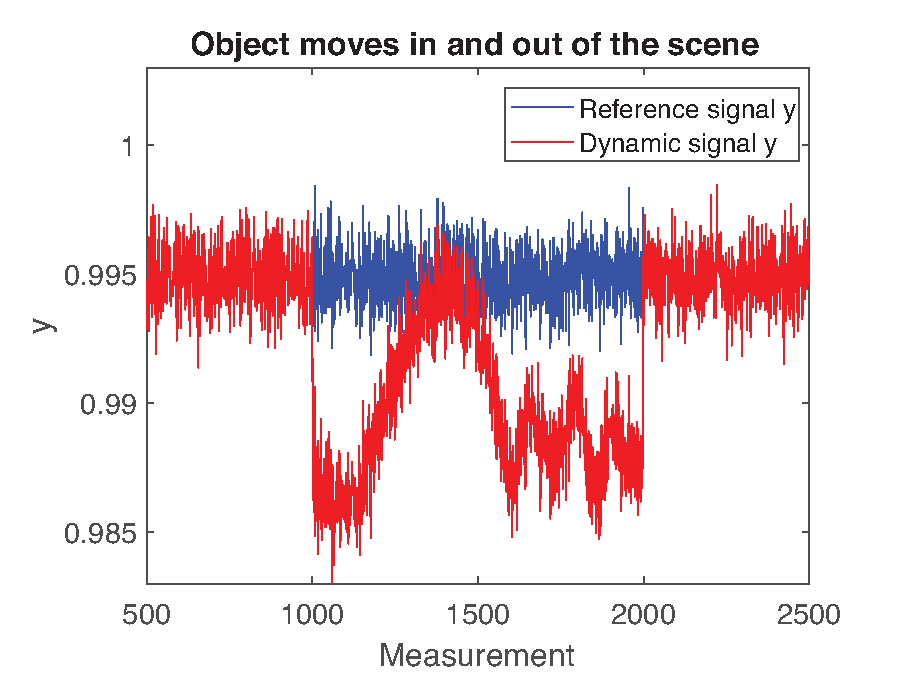
\includegraphics[width = \textwidth]{result/dynamic/fly/flyby_plot_win1.eps}
    \subcaption{}
    \label{fig:fly_sig_2}
\end{minipage}
    \caption{(a) Pertubated signal from large movement on top of reference signal. (b) Zoomed in view of some samples from figure (a).}
    \label{fig:fly_sig}
\end{figure}

As seen in figure~\ref{fig:fly_sig} the exact moment the object enters the scene the signal changes. This is because a completely new structure has entered the scene and therefore changing the DC level. It can also be noted that the object passed something which has approximately the same intensity as the background and therefore the DC signal almost comes back up to its original state for a brief moment.\\[0.1in] 

In figure~\ref{fig:fly_dyn} the effect of the moving object can be seen in the reconstructed image which has gained a lot of global noise. Note that the object passing trough can not be seen because there is more measurements with the background and the object moving creating uncertainty in the whole image.   

\begin{figure}[H]
    \centering
\begin{minipage}[t]{0.32\textwidth}
    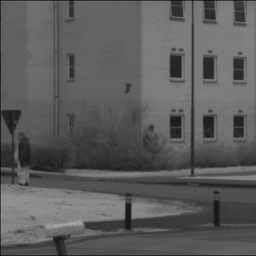
\includegraphics[width=1\textwidth]{result/dynamic/fly/flyby_1sec_org.png}
    \subcaption{}
    \label{fig:fly_1}
\end{minipage}
\begin{minipage}[t]{0.32\textwidth}
    
\includegraphics[width = \textwidth]{result/dynamic/fly/flyby_1sec_ref.png}
    \subcaption{}
    \label{fig:fly_2}
\end{minipage}
\begin{minipage}[t]{0.32\textwidth}
    
\includegraphics[width = \textwidth]{result/dynamic/fly/flyby_1sec_res_psnr_23_snr_18_sssim_58.png}
    \subcaption{}
    \label{fig:fly_3}
\end{minipage}
    \caption{The results of large movement on a reconstructed image, sub sampled at 30\%. (a) Original reference image. (b) Reference image reconstructed from the original image without movement. (c) Reconstructed image from a scene with object passing trough.}
    \label{fig:fly_dyn}
\end{figure}

In table~\ref{tab:fly_dyn} the results from calculating PSNR and SSIM between the reconstructed images is presented. It can be observed that the image has been effected heavily by the movement. 


\begin{table}[H]
    \centering
  \begin{tabular}{ | l | l | l |}
    \hline
    Peak SNR & SNR & SSIM \\ \hline
    23 & 18 & 58 \\ 
    \hline
  \end{tabular}
      \caption{Effects comparing non perturbed reconstructed image against reconstructed image with local movement}
    \label{tab:fly_dyn}
\end{table}


Obviously in this context the samples with movement is very easy to spot and the easiest fix would be to just remove those measurements, reconstructing an image with fewer measurements. The resulting image would not be as good as the image in figure~\ref{fig:fly_2} but it would not be contain the noise present in figure~\ref{fig:fly_3}.\\[0.1in]



%%%%%%%%%%%% Third %%%%%%%%%%%%%%%

The third scenario i luminance change in the scene caused by clouds occludes the sun or the light intensity from the lights is not constant. This scenario is modeled by adding or subtracting the global intensity in the image over the measurements. 

\begin{figure}[H]
    \centering
\begin{minipage}[t]{0.245\textwidth}
    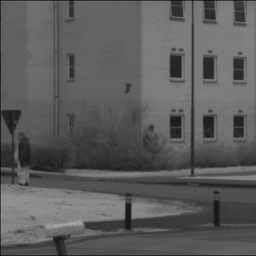
\includegraphics[width=1\textwidth]{result/dynamic/lum/intense_change_org.png}
    \subcaption{Original reference image}
    \label{fig:lum_1}
\end{minipage}
\begin{minipage}[t]{0.245\textwidth}
    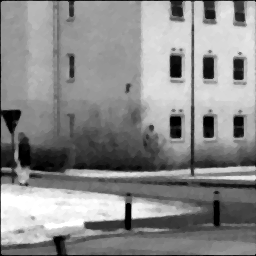
\includegraphics[width = \textwidth]{result/dynamic/lum/intense_change.png}
    \subcaption{Reconstructed $30\%$ image from reference image without movement}
    \label{fig:lum_2}
\end{minipage}
\begin{minipage}[t]{0.245\textwidth}
    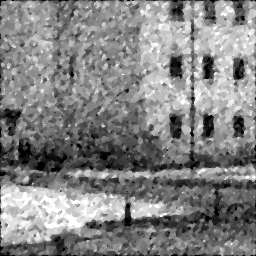
\includegraphics[width = \textwidth]{result/dynamic/lum/intense_change_psnr_19_snr_14_sssim_38.png}
    \subcaption{Reconstructed $30\%$ image with global luminance change}
    \label{fig:lum_3}
\end{minipage}
\begin{minipage}[t]{0.245\textwidth}
    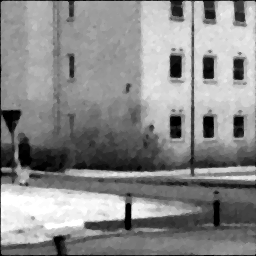
\includegraphics[width = \textwidth]{result/dynamic/lum/intense_change_movemean_psnr_33_snr_29_sssim_93.png}
    \subcaption{Reconstructed $30\%$ image with mean subtraction}
    \label{fig:lum_4}
\end{minipage}
    \caption{Global luminance change in scene.}
    \label{fig:lum_dyn}
\end{figure}


The difference between figure~\ref{fig:lum_2} and \ref{fig:lum_3} is visible with the naked eye, A global noise arises in the image, but as seen in figure~\ref{fig:lum_4} the effect can be suppressed explained under figure~\ref{fig:lum_sig}. In table~\ref{tab:fly_dyn}...


\begin{table}[H]
    \centering
  \begin{tabular}{ | l | l | l | l |}
    \hline
     & Peak SNR & SNR & SSIM \\ \hline
    Perturbed signal & 19 & 14 & 38 \\ \hline
    Mean subtracted signal & 33 & 29 & 93 \\
    \hline
  \end{tabular}
      \caption{Effects comparing non perturbed reconstructed image against reconstructed image with global luminance change}
    \label{tab:lum_dyn}
\end{table}


Commenting the result from the table... In figure~\ref{fig:lum_sig} the effects of global luminance is shown plotted against the non perturbed signal.\\[0.1in]


\begin{figure}[H]
    \centering
\begin{minipage}[t]{0.55\textwidth}
    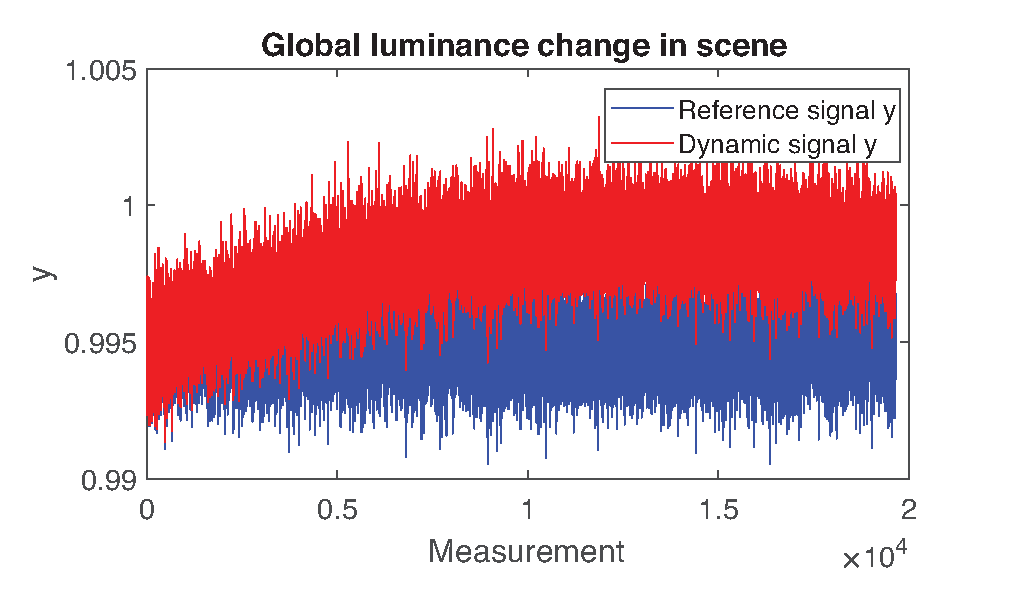
\includegraphics[width=1\textwidth]{result/dynamic/lum/intense_change1.eps}
    \subcaption{Signal.}
    \label{fig:lum_sig_1}
\end{minipage}
\begin{minipage}[t]{0.44\textwidth}
    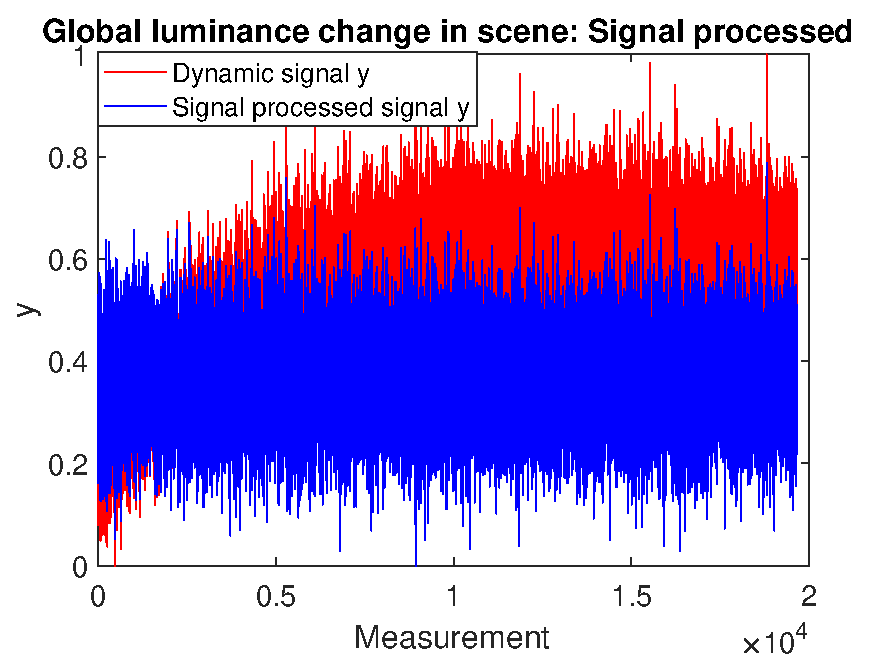
\includegraphics[width = \textwidth]{result/dynamic/lum/intense_change_sp.eps}
    \subcaption{Zoomed in view of the signal.}
    \label{fig:lum_sig_2}
\end{minipage}
\begin{minipage}[t]{0.495\textwidth}
    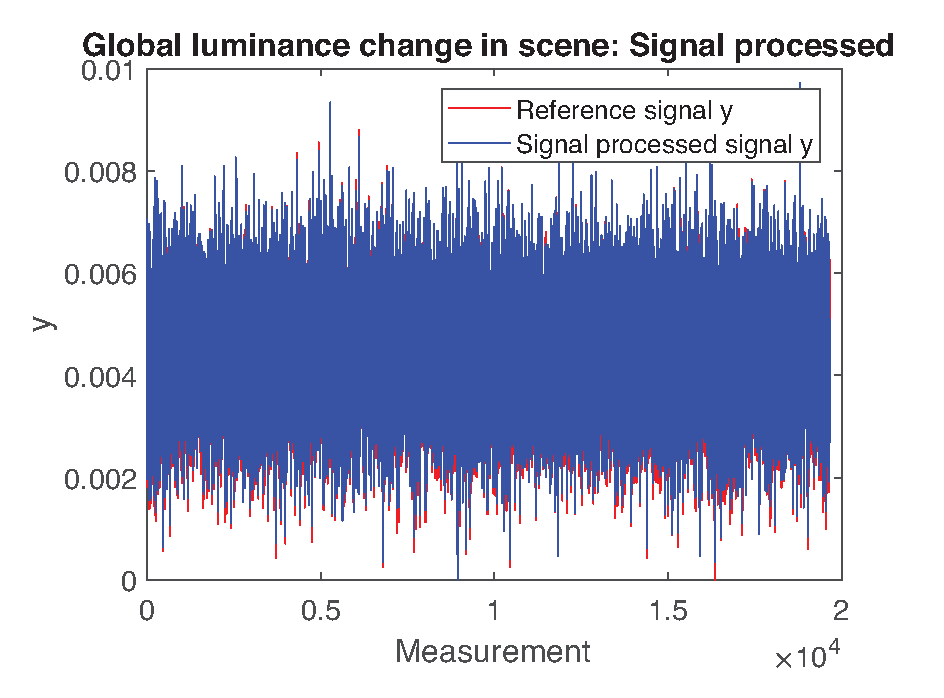
\includegraphics[width=1\textwidth]{result/dynamic/lum/intense_change_sp_ref1.eps}
    \subcaption{Signal.}
    \label{fig:lum_sig_3}
\end{minipage}
\begin{minipage}[t]{0.495\textwidth}
    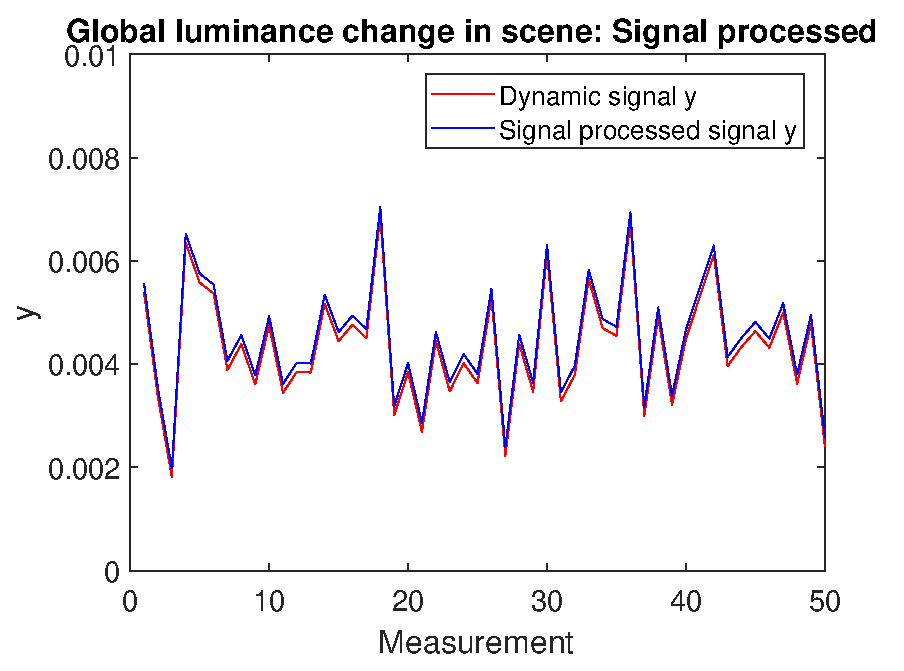
\includegraphics[width = \textwidth]{result/dynamic/lum/intense_change_sp_ref_win.eps}
    \subcaption{Zoomed in view of the signal.}
    \label{fig:lum_sig_4}
\end{minipage}
    \caption{Global movement, acquired signal}
    \label{fig:lum_sig}
\end{figure}

\begin{itemize}
    \item Dynamic signal v. Reference signal
    \item Dynamic signal v. Mean subtracted signal
    \item Reference signal v. Mean subtracted signal
    \item Comment on the window, pretty good.
    \item Can be detected with the knowledge that the signal should be stationary. Signal process the signal to look like a stationary signal.
\end{itemize}
